\documentclass[tikz,border=10pt]{standalone}
\usepackage{tikz}
\usetikzlibrary {angles,quotes,arrows.meta}
\usetikzlibrary{decorations.markings}
\tikzset{%
  ->-/.style={decoration={markings, mark=at position 0.2 with {\arrow{>[scale = 1, length=3]}}},
              postaction={decorate}},
}

\begin{document}
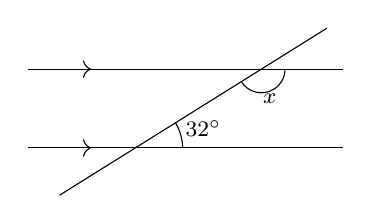
\begin{tikzpicture}[scale = 1]
    \coordinate (A) at (0,0);
    \coordinate (B) at (4,0);
    \coordinate (C) at (0,1);
    \coordinate (D) at ( 4,1);
    \coordinate (E) at (0.4,-0.6);
    \path (E) -- ++(32:4cm) coordinate (F);

    %parallel lines
    \draw[->-] (A) -- (B);
    \draw[->-] (C) -- (D);
    
    \coordinate (X) at (intersection cs:first line={(A)--(B)}, second line={(E)--(F)});
    \coordinate (Y) at (intersection cs:first line={(C)--(D)}, second line={(E)--(F)});
    
    %traversal line EF
    \draw (E) -- (F);
    % Draw the angle between lines
    \pic [draw, "\footnotesize $32^\circ$ ", angle eccentricity=1.5, angle radius=0.6cm] {angle = B--X--Y};
    \pic [draw, "\footnotesize $x$ ", angle eccentricity=1.3, angle radius=0.3cm] {angle = X--Y--D};
    
\end{tikzpicture}

\end{document}
